% Provenance (never printed): see sources/outline_sources.md (Year 1: morphology,
% gravity, heat flow and seismicity of a subduction zone; accretionary and erosive
% margins; slab geometry; volcanic arcs). Kuril map, section and numbers from
% figdata/bachelor-1/slab_seismicity.py; exercise and problem values in the Book 3
% scratch calculator calc/ch14.py.
\chapter{सक्रिय किनारे}\label{ch:b1:active-margins}

11 मार्च 2011 को, स्थानीय समय 14:46 बजे, उत्तर-पूर्वी जापान के तट से दूर प्लेट-सीमा खाई के साथ लगभग \qty{400}{km} पर और उसकी \omterm{def:b1:geological-maps:attitude}{नति} के नीचे \qty{150}{km} तक टूट गई। भ्रंश 50 से \qty{60}{m} तक सरका, अधिकांश भाग अधिकेंद्र के \omterm{def:b1:geological-maps:attitude}{नति} की ओर ऊपर, जापान खाई की दिशा में; ज़मीन पर तट क्षैतिज रूप से खिसका और धँस गया। वहाँ धँसने वाली प्लेट, प्रशांत प्लेट, जापान के नीचे एक ऐसे तल के अनुदिश नीचे जाती है जिसे भूकंप सैकड़ों किलोमीटर नीचे तक रेखांकित करते हैं; और जहाँ वह तल लगभग सौ किलोमीटर गहराई पर है, वहाँ ज्वालामुखियों की एक पंक्ति तट के समांतर चलती है। यह अध्याय ऐसे किनारे को उसके आकार, गुरुत्व, \omterm{def:b1:heat-budget:heat-flow}{ऊष्मा-प्रवाह} और, सबसे बढ़कर, उसके भूकंपों से पढ़ता है।
% ledger: usgs:tohoku, wada:decoupling

\begin{recall}
महासागरीय \omterm{def:b1:layered-earth:lithosphere}{स्थलमंडल} खाइयों और भूकंपों के झुके क्षेत्रों से चिह्नित निमज्जन-क्षेत्रों पर \omterm{def:b1:layered-earth:layers}{प्रावार} में वापस धँसता है, और पुराना \omterm{def:b1:layered-earth:lithosphere}{स्थलमंडल} अपने ही भार से धँसता है (पुस्तक 2, कक्षा 11); धँसती प्लेट का पानी उसके ऊपर के \omterm{def:b1:layered-earth:layers}{प्रावार} का गलन-तापमान घटाता है (पुस्तक 2, कक्षा 12)। ऊष्मा एक दूरी $L$ पर लगभग $L^2/\kappa$ के क्रम के समय में विसरित होती है (\cref{ch:b1:heat-budget}); घनत्व $\rho$ और मोटाई $h$ की एक अनंत पट्टी $2\pi G\rho h$ से आकर्षित करती है (\cref{ch:b1:isostasy-gravity}); प्लेटें यूलर ध्रुवों के परितः घूमती हैं (\cref{ch:b1:plate-kinematics}); महासागर-तल का \omterm{def:b1:heat-budget:heat-flow}{ऊष्मा-प्रवाह} उसकी आयु के व्युत्क्रम वर्गमूल से गिरता है (\cref{ch:b1:rifts-ridges-margins})।
\end{recall}

\section{एक सक्रिय किनारे की शारीरिक रचना}\label{sec:b1:active-margins:anatomy}

\begin{definition}[सक्रिय किनारा, महासागरीय खाई, फ़ोरआर्क, बैक-आर्क द्रोणी]\label{def:b1:active-margins:active-margin}
एक \emph{सक्रिय किनारा}\index{सक्रिय किनारा} एक अभिसारी प्लेट-सीमा है जिस पर महासागरीय \omterm{def:b1:layered-earth:lithosphere}{स्थलमंडल} दूसरी प्लेट के नीचे धँसता है, या तो एक महाद्वीप के नीचे या दूसरी महासागरीय प्लेट के नीचे। एक \emph{महासागरीय खाई}\index{महासागरीय खाई} समुद्र-तल का लंबा, संकरा, V-आकार का अवनमन है जिसके अनुदिश धँसती प्लेट दूसरी के नीचे मुड़ती है। \emph{फ़ोरआर्क}\index{फ़ोरआर्क} ऊपरी प्लेट का वह भाग है जो खाई और ज्वालामुखियों की पंक्ति के बीच है। एक \emph{बैक-आर्क द्रोणी}\index{बैक-आर्क द्रोणी} ज्वालामुखियों के पीछे, खाई से दूर की ओर, एक द्रोणी है जहाँ ऊपरी प्लेट खिंचती है और नई \omterm{def:b1:rifts-ridges-margins:oceanic-crust}{महासागरीय भूपर्पटी} बन सकती है।
\end{definition}

खाइयाँ महासागरों की सबसे गहरी जगहें हैं, और सबसे गहरी चैलेंजर डीप है, मारियाना खाई में। कुरील खाई के आर-पार तल अतल मैदान पर लगभग \qty{5200}{m} से अक्ष पर \qty{8700}{m} तक गिरता है, लगभग \qty{3.5}{km} नीचे, और खाई केवल दसियों किलोमीटर चौड़ी है (चित्र \cref{sec:b1:active-margins:gravity-heat} में)। पृथ्वी के अभिसारी किनारे कुल मिलाकर लगभग \qty{55000}{km} मापते हैं; प्लेट-सीमाओं के एक अंकीय प्रतिरूप में निमज्जन-सीमाएँ लगभग \qty{51000}{km} जुड़ती हैं, जबकि प्रसारी कटक लगभग \qty{67000}{km}।
% ledger: data:b3-grav-kuril (trench_gravity.py values), stern:subduction, data:pb2002 (ridge_budget.py)

खाई के समुद्री ओर प्लेट धँसने से पहले थोड़ा उठती है, एक चौड़े, नीचे बाहरी उभार में। वहाँ प्लेट मुड़ी है, और उसका ऊपरी भाग खिंचा है: बाहरी उभारों पर सामान्य भ्रंशन के भूकंप आते हैं। बाहरी उभार की चौड़ाई एक प्रत्यास्थ प्लेट के मोड़ से मेल खाती है; \omterm{def:b1:layered-earth:lithosphere}{स्थलमंडल} का यह मोड़ पुस्तक 5 में पढ़ा जाता है। खाई स्वयं वह जगह है जहाँ सघन धँसती प्लेट का भार उसके अग्र किनारे को नीचे खींचता है।

\begin{definition}[निमज्जित स्लैब]\label{def:b1:active-margins:slab}
\emph{निमज्जित स्लैब}\index{निमज्जित स्लैब} धँसती प्लेट का वह भाग है जो पहले ही \omterm{def:b1:layered-earth:layers}{प्रावार} में नीचे जा चुका है: महासागरीय \omterm{def:b1:layered-earth:lithosphere}{स्थलमंडल} की एक चादर, अपनी \omterm{def:b1:layered-earth:layers}{भूपर्पटी} ऊपर, खाई से लेकर कई सौ किलोमीटर गहराई तक ऊपरी प्लेट के नीचे झुकी हुई।
\end{definition}

ऊपरी प्लेट खाई के समांतर पट्टियों में कटी है (नीचे का चित्र): \omterm{def:b1:active-margins:active-margin}{फ़ोरआर्क}, जिसके सामने प्रायः खुरची गई अवसादों का ढेर और पीछे एक अवसादी द्रोणी होती है; \omterm{def:b1:active-margins:volcanic-arc}{ज्वालामुखी चाप}; और कुछ चापों के पीछे, एक \omterm{def:b1:active-margins:active-margin}{बैक-आर्क द्रोणी} और उसके परे एक पुराना, विलुप्त चाप। स्लैब और ऊपरी प्लेट के बीच \omterm{def:b1:layered-earth:layers}{प्रावार} का एक पच्चर है, जो स्लैब के शीर्ष के साथ नीचे खींचा जाता है।

\begin{omfigure}
\begin{tikzpicture}[x=0.01667cm, y=0.01667cm, font=\scriptsize,
  lbl/.style={fill=white, fill opacity=0.8, text opacity=1, inner sep=1pt}]
\begin{scope}
\clip (-150,-330) rectangle (650,55);
% mantle and sea water
\fill[orange!12] (-150,-330) rectangle (650,15);
\fill[omSea!45] (-150,15) rectangle (650,0);
% incoming plate and slab: top dips 25 deg to 50 km, then 45 deg; 100 km thick
\fill[omLithBasalt!55] (-150,4) -- (-80,4) .. controls (-60,7) and (-40,7) .. (-25,4) -- (0,0)
  -- (107.2,-50) -- (420,-363) -- (349,-434) -- (48.9,-133.1) -- (-22.1,-100) -- (-150,-100) -- cycle;
\draw[omSea!50!black, line width=1.6pt] (-150,4) -- (-80,4) .. controls (-60,7) and (-40,7) .. (-25,4) -- (0,0) -- (107.2,-50) -- (420,-363);
% overriding plate
\fill[brown!28] (0,0) -- (12,3) -- (45,8) -- (60,10) -- (140,10) -- (150,12) -- (184,12) -- (230,9)
  -- (300,7) -- (395,6) -- (410,3) -- (420,2) -- (430,3) -- (445,6) -- (540,7) -- (560,14) -- (590,14)
  -- (610,10) -- (650,10) -- (650,-60) -- (520,-55) -- (445,-25) -- (420,-15) -- (395,-25) -- (320,-55)
  -- (250,-60) -- (117.2,-60) -- (107.2,-50) -- cycle;
% accretionary prism and forearc basin
\fill[yellow!55] (0,0) -- (12,3) -- (45,8) -- (60,10) -- (60,-28) -- cycle;
\draw[black!45, line width=0.3pt] (14,-3) -- (24,5) (28,-7) -- (38,6) (42,-14) -- (52,8);
\fill[yellow!30] (68,10) -- (132,10) -- (122,4) -- (78,4) -- cycle;
% arc volcano
\fill[black!60] (150,12) -- (167,26) -- (184,12) -- cycle;
% an isotherm: a cold tongue down the slab
\draw[omDef, dashed, line width=0.6pt] (-150,-82) -- (-30,-82) -- (40,-118) -- (300,-318)
  -- (232,-200) -- (150,-112) .. controls (130,-80) and (180,-72) .. (260,-72) -- (650,-72);
% mantle wedge flow
\draw[->, black!60, line width=0.5pt] (600,-130) .. controls (450,-135) and (300,-125) .. (215,-150)
  .. controls (205,-160) and (240,-185) .. (300,-235);
% water and melt
\foreach \x/\z in {150/-93, 172/-115, 194/-137}
  \draw[->, blue!70!black, line width=0.5pt] (\x,\z) -- (\x-6,\z+28);
\draw[red!75!black, line width=0.8pt, decorate, decoration={snake, amplitude=1.2, segment length=6}] (167,-100) -- (167,12);
% earthquakes
\foreach \x/\z in {20/-12, 45/-22, 70/-34, 95/-45, 60/-40, 85/-58, 120/-70, 135/-85, 150/-104,
  165/-112, 185/-140, 205/-150, 225/-175, 248/-195, 270/-216, 290/-242, 312/-262, 330/-282, 350/-300, 365/-318}
  \fill[black] (\x,\z) circle[radius=0.9pt];
% the 100-km level beneath the arc
\draw[black!70, densely dotted] (90,-100) -- (260,-100);
\draw[black!70, densely dotted] (167,12) -- (167,-110);
\end{scope}
\draw[black!70] (-150,-330) rectangle (650,55);
  \node[lbl, anchor=south] at (-85,15) {बाहरी उभार};
  \node[lbl, anchor=south] at (0,15) {खाई};
  \node[lbl, anchor=west] (pr) at (75,-28) {संचयी प्रिज़्म};
\draw[black!70] (pr.west) -- (38,-6);
  \node[lbl, anchor=south] at (88,15) {फ़ोरआर्क};
  \node[lbl, anchor=south] at (185,27) {ज्वालामुखी चाप};
  \node[lbl, anchor=south] at (420,15) {बैक-आर्क द्रोणी};
  \node[lbl, anchor=south] at (575,15) {अवशेष चाप};
  \node[lbl, anchor=west] at (-140,-50) {महासागरीय स्थलमंडल};
  \node[lbl, anchor=east] (sl) at (120,-262) {निमज्जित स्लैब};
\draw[black!70] (sl.east) -- (205,-262);
  \node[lbl, anchor=west] (wb) at (420,-265) {वादाती–बेनीऑफ़ क्षेत्र};
\draw[black!70] (wb.west) -- (318,-266);
  \node[lbl] at (430,-170) {प्रावार-पच्चर};
  \node[lbl] at (575,-30) {ऊपरी प्लेट};
  \node[lbl, anchor=west, text=blue!70!black] at (212,-98) {पानी};
  \node[lbl, anchor=east] at (88,-100) {\qty{100}{km} गहरा};
  \node[lbl, anchor=west, text=omDef] at (450,-95) {एक समतापीय रेखा};
  \node[lbl, anchor=west] at (-140,-300) {प्रावार};
\draw[line width=1pt] (500,-310) -- (600,-310) node[midway, above] {\qty{100}{km}};
\end{tikzpicture}
\par\smallskip{\small एक निमज्जन-क्षेत्र काट में (योजनाबद्ध: \omterm{def:b1:layered-earth:lithosphere}{स्थलमंडल} और स्लैब को मापनी पट्टी तक खींचा गया, समुद्र-तल से ऊपर का उच्चावच बहुत बढ़ाकर)। स्लैब \omterm{def:b1:active-margins:active-margin}{फ़ोरआर्क} के नीचे हल्के झुकता है और नीचे अधिक तीखा; \omterm{def:b1:active-margins:volcanic-arc}{ज्वालामुखी चाप} वहाँ के ऊपर खड़ा है जहाँ स्लैब का शीर्ष लगभग \qty{100}{km} गहरा है। ठंडा स्लैब अपनी समतापीय रेखाएँ \omterm{def:b1:layered-earth:layers}{प्रावार} में नीचे खींचता है (बिंदुकित: एक समतापीय रेखा), और पच्चर का \omterm{def:b1:layered-earth:layers}{प्रावार} उसके साथ नीचे खींचा जाता है। बिंदु: भूकंप, खाई के निकट प्लेट-सीमा पर और नीचे स्लैब के भीतर। स्लैब से मुक्त पानी पच्चर में ऊपर उठता है; मैग्मा चाप की ओर उठता है।}
\label{fig:b1:active-margins:section}
\end{omfigure}

इसी डिजिटल प्रतिरूप पर, हर वर्ष लगभग \qty{2.7}{km^2} महासागर-तल निमज्जन-सीमाओं से नीचे जाता है, कटकों पर बने \qty{3.0}{km^2} के निकट (\cref{ch:b1:rifts-ridges-margins})। ऐसे प्रतिरूप की परिशुद्धता के भीतर, जो प्लेट-सीमा क्षेत्रों के धीमे विरूपण को छोड़ देता है, महासागर-तल उतनी ही तेज़ी से नष्ट होता है जितनी तेज़ी से बनता है, और पृथ्वी की सतह अपना आकार बनाए रखती है।
% ledger: data:pb2002 (ridge_budget.py: consumed 2.74, made 3.01 km2/yr)

\section{गुरुत्व और ऊष्मा-प्रवाह}\label{sec:b1:active-margins:gravity-heat}

फ़ेलिक्स वेनिंग मायनेज़ ने खाइयों के किनारे ऋणात्मक गुरुत्व विसंगतियों की लंबी, संकरी पेटियाँ पाईं (\cref{ch:b1:isostasy-gravity})। उपग्रह उन्हें अब हर जगह समुद्र में मानचित्रित करते हैं। कुरील खाई के आर-पार (नीचे का चित्र) \omterm{def:b1:isostasy-gravity:anomalies}{मुक्त-वायु विसंगति} बाहरी उभार पर लगभग \qty{40}{\milli\gal} तक उठती है, खाई पर \qty{-260}{\milli\gal} तक गिरती है, और \omterm{def:b1:active-margins:active-margin}{फ़ोरआर्क} और चाप के द्वीपों पर फिर प्रबल रूप से धनात्मक है।
% ledger: egs:vening-meinesz, data:b3-grav-kuril (trench_gravity.py values: rise 38 mGal at -155 km, low -260 at 0, high 218 at 160 km)

खाई की विसंगति का आकार बताता है कि खाई कैसे टिकी है। मान लीजिए खाई, अपने चारों ओर के तल से \qty{3.5}{km} गहरी, बिल्कुल प्रतिपूरित नहीं है: जहाँ खाई है, घनत्व लगभग \qty{2700}{kg.m^{-3}} की \qty{3.5}{km} चट्टान समुद्री पानी से बदल दी गई है। बूगेर पट्टी (\cref{prop:b1:isostasy-gravity:slab}) द्वारा वहाँ गुरुत्व इतना कम होगा
\[
  2\pi G\,\Delta\rho\,h = 2\pi \times \num{6.674e-11} \times 1700 \times 3500
  \approx \qty{2.5e-3}{m.s^{-2}} = \qty{250}{\milli\gal} .
\]
उस मात्रा का प्रेक्षित निम्न के बराबर आकार है। खाई इसलिए समस्थैतिक साम्य में नहीं है: वह एक दबाया गया अवनमन है, मुड़ी प्लेट की मज़बूती और स्लैब के खिंचाव से, नीचे के \omterm{def:b1:layered-earth:layers}{प्रावार} की उत्प्लावकता के विरुद्ध टिका हुआ। (दसियों किलोमीटर चौड़ी खाई एक अनंत स्लैब से कम आकर्षित करती है, इसलिए उसमें अकेला पानी इससे कुछ कम देता है; शेष कमी गहरे है, जहाँ पूरी मुड़ी प्लेट, उसकी हल्की \omterm{def:b1:layered-earth:layers}{भूपर्पटी} सहित, \omterm{def:b1:layered-earth:layers}{प्रावार} में दबाई जाती है: अभ्यास~\ref{exo:b1:active-margins:1})।

\begin{omfigure}
\begin{tikzpicture}
\begin{axis}[omrecord, name=grav, width=0.86\linewidth, height=4.6cm, xmin=-250, xmax=450,
  ymin=-300, ymax=260, ylabel={मुक्त-वायु (\unit{\milli\gal})}, ylabel style={at={(-0.075,0.5)}}, xticklabels={},
  ytick={-200,-100,0,100,200}, clip=false]
% computed in figdata/bachelor-1/trench_gravity.py; ledger: data:b3-grav-kuril
\addplot[black!30, forget plot] coordinates {(-250,0) (450,0)};
\addplot[omDef, line width=1pt] table[x=x, y=faa] {figdata/out/bachelor-1-trench_gravity-profile.dat};
\draw[black!50, densely dotted] (axis cs:0,-300) -- (axis cs:0,260) (axis cs:164,-300) -- (axis cs:164,260);
\node[font=\scriptsize, anchor=south] at (axis cs:-155,45) {बाहरी उभार, $+38$};
\node[font=\scriptsize, anchor=west] at (axis cs:12,-262) {खाई, $-260$};
\node[font=\scriptsize, anchor=south west] at (axis cs:200,140) {फ़ोरआर्क और चाप};
\end{axis}
\begin{axis}[omrecord, at={(grav.south)}, anchor=north, yshift=-0.45cm, width=0.86\linewidth, height=4.6cm,
  xmin=-250, xmax=450, ymin=20, ymax=100, ylabel={ऊष्मा (\unit{mW.m^{-2}})}, ylabel style={at={(-0.075,0.5)}},
  xlabel={खाई से दूरी, ऊपरी प्लेट की ओर (\unit{km})}, clip=false]
% schematic; levels from the ledger: parsons:plate-model (11.3/sqrt(122) x 41.84 = 42.8 mW/m2 for the
% 122-Myr Kuril plate), hyndman:backarc (70-85); the forearc low is drawn without a value (wada:decoupling)
\addplot[fill=omDef!15, draw=none, forget plot] coordinates {(190,70) (450,70) (450,85) (190,85)} -- cycle;
\addplot[omProp!80!black, line width=1pt, smooth, tension=0.5] coordinates {(-250,43) (-60,43) (-10,41) (30,36) (120,36)
  (150,48) (180,76) (230,78) (450,78)};
\draw[black!50, densely dotted] (axis cs:0,20) -- (axis cs:0,100) (axis cs:164,20) -- (axis cs:164,100);
\node[font=\scriptsize, anchor=south] at (axis cs:-130,44) {पुराना महासागर-तल, लगभग 43};
\node[font=\scriptsize, anchor=north] at (axis cs:75,34) {फ़ोरआर्क: निम्न};
\node[font=\scriptsize, anchor=south] at (axis cs:320,85) {चाप और बैक-आर्क, 70 से 85};
\node[font=\scriptsize, anchor=north west] at (axis cs:3,99) {खाई};
\node[font=\scriptsize, anchor=north west] at (axis cs:167,99) {चाप};
\end{axis}
\end{tikzpicture}
\par\smallskip{\small सबडक्शन क्षेत्र पर गुरुत्व और \omterm{def:b1:heat-budget:heat-flow}{ऊष्मा-प्रवाह}। ऊपर: उपग्रह द्वारा कुरील खाई के आर-पार मापी गई मुक्त-वायु \omterm{def:b1:isostasy-gravity:anomalies}{गुरुत्व विसंगति}, चित्र के परिच्छेद के साथ \cref{sec:b1:active-margins:seismicity} में: बाहरी उभार पर \qty{38}{\milli\gal}, खाई पर \qty{-260}{\milli\gal}, \omterm{def:b1:active-margins:active-margin}{फ़ोरआर्क} और द्वीपों पर प्रबल रूप से धनात्मक। नीचे: \omterm{def:b1:heat-budget:heat-flow}{ऊष्मा-प्रवाह}, एक योजनाबद्ध परिच्छेद: पुराने महासागर-तल पर लगभग \qty{43}{mW.m^{-2}}, \omterm{def:b1:active-margins:active-margin}{फ़ोरआर्क} के ऊपर निम्न, चाप और बैक-आर्क पर औसतन \qty{70} से \qty{85}{mW.m^{-2}}। बिंदुकित: खाई और ज्वालामुखी अग्र। आँकड़े: Scripps Institution of Oceanography समुद्री गुरुत्व प्रतिरूप (Sandwell और अन्य, 2014)।}
\label{fig:b1:active-margins:profiles}
\end{omfigure}

\omterm{def:b1:heat-budget:heat-flow}{ऊष्मा-प्रवाह} वही कहानी दूसरी ओर से बताता है। पुराना महासागर-तल जो एक खाई तक आता है, थोड़ी ऊष्मा खोता है: \qty{122}{Myr} पुरानी कुरील प्लेट के लिए \cref{ch:b1:rifts-ridges-margins} के नियम से लगभग \qty{43}{mW.m^{-2}}। \omterm{def:b1:active-margins:active-margin}{फ़ोरआर्क} के ऊपर प्रवाह और भी कम है: उसके नीचे का ठंडा स्लैब ऊपर से ऊष्मा लेता है, और \omterm{def:b1:active-margins:active-margin}{फ़ोरआर्क} के नीचे का \omterm{def:b1:layered-earth:layers}{प्रावार} ठंडा और स्थिर है। चाप और बैक-आर्क के ऊपर वह ऊँचा है, औसतन 70 से \qty{85}{mW.m^{-2}}, महाद्वीपों के पुराने आंतरिक भागों के प्रवाह (लगभग \qty{40}{mW.m^{-2}}) का दोगुना। एक सक्रिय \omterm{def:b1:active-margins:volcanic-arc}{ज्वालामुखी चाप} को लगभग \qty{100}{km} नीचे लगभग \qty{1200}{\celsius} पर एक प्रावार-पच्चर चाहिए; उसके पीछे पूरा बैक-आर्क गरम है, केवल 50 से \qty{60}{km} मोटे \omterm{def:b1:layered-earth:lithosphere}{स्थलमंडल} के साथ और उसका \omterm{def:b1:layered-earth:discontinuity}{मोहो} 800 से \qty{900}{\celsius} पर।
% ledger: parsons:plate-model (11.3/sqrt(122) x 41.84 = 42.8), wada:decoupling, hyndman:backarc

स्लैब ठंडा क्यों रहता है? वह उससे तेज़ धँसता है जितनी तेज़ी से वह गरम हो सकता है। \cref{sec:b1:active-margins:seismicity} का कुरील स्लैब लगभग \qty{82}{mm} प्रति वर्ष पर प्रवेश करता है और \ang{45} पर झुकता है: वह $600/\sin\ang{45} \approx \qty{850}{km}$ के पथ के बाद, लगभग दस मिलियन वर्षों में, \qty{600}{km} तक पहुँचता है। चालन के समय-पैमाने (\cref{prop:b1:heat-budget:timescale}) से, \omterm{def:b1:layered-earth:layers}{प्रावार} की ऊष्मा \qty{100}{km} मोटे स्लैब के मध्य तक \qty{50}{km} पार करने में
\[
  \tau = \frac{L^2}{\kappa} = \frac{(\qty{5e4}{m})^2}{\qty{e-6}{m^2.s^{-1}}}
  = \qty{2.5e15}{s} \approx \qty{80}{Myr},
\]
लगभग आठ गुना अधिक समय लगता है। स्लैब का केंद्र \qty{600}{km} पर लगभग उतना ही ठंडा पहुँचता है जितना खाई पर था, और समतापीय रेखाएँ उसके साथ नीचे खिंचती हैं, जैसा ऊपर सबडक्शन क्षेत्र का परिच्छेद दिखाता है।
% values (slab_seismicity.py): vel_normal 81.66 mm/yr, dip 44.9; calc/ch14.py

\section{भूकंप और स्लैब का आकार}\label{sec:b1:active-margins:seismicity}

\begin{definition}[वादाती–बेनीऑफ़ क्षेत्र]\label{def:b1:active-margins:wadati-benioff}
एक \emph{वादाती–बेनीऑफ़ क्षेत्र}\index{वादाती–बेनीऑफ़ क्षेत्र} भूकंपों का झुका क्षेत्र है जो एक खाई के निकट शुरू होता है और ऊपरी प्लेट के नीचे गहरा होता है, लगभग \qty{700}{km} तक: वह \omterm{def:b1:active-margins:slab}{धँसते स्लैब} की रूपरेखा बनाता है।
\end{definition}
% ledger: usgs:deepest

उसके भूकंप दो प्रकार के हैं। कुछ दसियों किलोमीटर तक वे प्लेट-सीमा पर ही होते हैं, वह मंद रूप से झुका दोष जिसके अनुदिश दोनों प्लेटें एक-दूसरे को सरकाती हैं; पृथ्वी के सबसे बड़े भूकंप, जैसे 2011 का जापान के तट से दूर वाला, इसी दोष को तोड़ते हैं। गहरे भूकंप स्लैब के भीतर होते हैं, जो अकेला अब भी तनाव संचित करने के लिए पर्याप्त ठंडा है। सबसे गहरी गहराइयों पर स्लैब को भी टूटने के बजाय बहना चाहिए, और गहरे भूकंप कितनी गहराई से शुरू होते हैं, यह अब भी विवादित है। सूची का सबसे गहरा भूकंप, परिमाण 4.2, 2004 में वानुआतु क्षेत्र के नीचे \qty{735.8}{km} पर आया। हर जाँचे गए निमज्जन-क्षेत्र में, मध्यवर्ती गहराइयों पर क्षेत्र दोहरा है: भूकंपों की दो परतें, पुरानी प्लेटों में एक-दूसरे से अधिक दूर।
% ledger: usgs:deepest, brudzinski:double, usgs:tohoku

कुरील द्वीप, होक्काइडो और कामचटका के बीच, एक ऐसे स्लैब के ऊपर बैठे हैं जिसे भूकंप खाई से लेकर \qty{600}{km} से अधिक तक रेखांकित करते हैं। वहाँ प्रशांत प्लेट, जो खाई तक पहुँचने पर लगभग 120 मिलियन वर्ष पुरानी है, ओखोत्स्क प्लेट के नीचे धँसती है (नीचे का मानचित्र)। 1976 से परिमाण 5 या अधिक के भूकंप स्लैब को मानचित्र में खींचते हैं: उथले खाई के साथ, मध्यवर्ती द्वीपों के नीचे, गहरे ओखोत्स्क सागर के नीचे। 24 मई 2013 को परिमाण 8.3 का भूकंप ओखोत्स्क सागर के नीचे \qty{598}{km} पर आया, उसी स्लैब में और उत्तर में; वह मॉस्को तक, लगभग \qty{6400}{km} दूर, महसूस किया गया।
% values (slab_seismicity.py): age_in 121.8 Myr (median of the cells 100-400 km seaward)
% ledger: data:b3-usgs-kuril, data:b2-seafloor-age, data:pb2002, usgs:okhotsk-2013

\begin{omfigure}
\begin{tikzpicture}
\begin{axis}[x=0.40cm, y=0.598cm, xmin=138, xmax=165, ymin=40, ymax=56,
  axis background/.style={fill=omSea!35}, axis on top,
  xtick={140,145,...,165}, ytick={40,45,...,55},
  xticklabel={$\pgfmathprintnumber{\tick}^\circ$E}, yticklabel={$\pgfmathprintnumber{\tick}^\circ$N},
  tick label style={font=\scriptsize}, grid=major, grid style={gray!25, line width=0.25pt},
  legend style={font=\scriptsize, at={(0.98,0.02)}, anchor=south east, cells={anchor=west}},
  clip=true]
% computed in figdata/bachelor-1/slab_seismicity.py; ledger: data:b3-usgs-kuril, data:gvp, data:pb2002
\addplot[fill=omLithAlluv, draw=black!45, line width=0.2pt, unbounded coords=jump, forget plot] table {figdata/out/bachelor-1-slab_seismicity-map-land.dat};
\addplot[only marks, mark=*, mark size=0.45pt, black!35] table {figdata/out/bachelor-1-slab_seismicity-map-qshallow.dat};
\addlegendentry{\qty{70}{km} से उथला}
\addplot[only marks, mark=*, mark size=0.8pt, orange!85!black] table {figdata/out/bachelor-1-slab_seismicity-map-qmid.dat};
\addlegendentry{70 से \qty{300}{km}}
\addplot[only marks, mark=*, mark size=1.0pt, omDef] table {figdata/out/bachelor-1-slab_seismicity-map-qdeep.dat};
\addlegendentry{\qty{300}{km} से गहरा}
\addplot[only marks, mark=triangle*, mark size=1.6pt, black, fill=red!70!black] table {figdata/out/bachelor-1-slab_seismicity-map-volc.dat};
\addlegendentry{होलोसीन ज्वालामुखी}
\addplot[black, line width=0.6pt, unbounded coords=jump, forget plot] table {figdata/out/bachelor-1-slab_seismicity-map-trench.dat};
\addplot[fill=black, draw=none, unbounded coords=jump, forget plot] table {figdata/out/bachelor-1-slab_seismicity-map-teeth.dat};
\addplot[omProp, line width=0.8pt, dashed, forget plot] table {figdata/out/bachelor-1-slab_seismicity-map-strip.dat};
\node[font=\scriptsize, fill=white, fill opacity=0.8, text opacity=1, inner sep=1pt] at (axis cs:147,54.3) {ओखोत्स्क सागर};
\node[font=\scriptsize, fill=white, fill opacity=0.8, text opacity=1, inner sep=1pt] at (axis cs:158.5,44) {प्रशांत प्लेट};
\node[font=\scriptsize, fill=white, fill opacity=0.8, text opacity=1, inner sep=1pt] at (axis cs:157.2,55.2) {कामचटका};
\node[font=\scriptsize, fill=white, fill opacity=0.8, text opacity=1, inner sep=1pt] at (axis cs:139.7,44.3) {होक्काइडो};
\node[font=\scriptsize, fill=white, fill opacity=0.8, text opacity=1, inner sep=1pt, rotate=40] at (axis cs:155.6,46.4) {कुरील खाई};
\node[font=\scriptsize, fill=white, fill opacity=0.8, text opacity=1, inner sep=1pt, text=omProp] at (axis cs:146.3,51.4) {परिच्छेद};
\end{axis}
\end{tikzpicture}
\par\smallskip{\small कुरील सबडक्शन क्षेत्र: 1976–2025 के परिमाण 5 या अधिक के भूकंप, गहराई के अनुसार रंगीन, और पिछले दस हज़ार वर्षों में सक्रिय ज्वालामुखी। खाई (ऊपरी प्लेट पर दाँत) और अगले चित्र का परिच्छेद-पट्टी (बिंदुकित, परिच्छेद रेखा के हर ओर \qty{150}{km})। डेटा: USGS भूकंप सूची; Smithsonian Global Volcanism Program; खाई Bird (2003) से; तट Natural Earth से।}
\label{fig:b1:active-margins:map}
\end{omfigure}

परिच्छेद में स्लैब देखने के लिए, खाई से शुरू होने वाली और उसके लंबवत ऊपरी प्लेट की ओर चलने वाली एक रेखा के \qty{150}{km} के भीतर के भूकंप रखिए, और हर एक को रेखा के अनुदिश उसकी दूरी $x$ और उसकी गहराई $z$ पर अंकित कीजिए (नीचे का चित्र)। बिंदु एक पट्टी बनाते हैं; वह सीधी रेखा जो उसका सबसे अच्छा अनुसरण करती है, न्यूनतम वर्गों से पाई जाती है।

\begin{method}[न्यूनतम वर्गों से स्लैब फ़िट करना]\label{met:b1:active-margins:lsq}
$n$ भूकंप, स्लैब के भीतर $(x_i, z_i)$ पर, दिए गए हैं:
\begin{enumerate}
  \item माध्य $\bar x = \frac1n\sum x_i$ और $\bar z = \frac1n\sum z_i$ परिकलित कीजिए;
  \item $S_{xx} = \sum (x_i - \bar x)^2 = \sum x_i^2 - n\bar x^2$ और
        $S_{xz} = \sum (x_i - \bar x)(z_i - \bar z) = \sum x_i z_i - n\bar x\bar z$ परिकलित कीजिए;
  \item स्लैब की रेखा $z = a + s x$ है, जहाँ $s = S_{xz}/S_{xx}$ और $a = \bar z - s\bar x$; उसकी \omterm{def:b1:geological-maps:attitude}{नति} $\delta = \arctan s$ है।
\end{enumerate}
\end{method}

यह रेखा निम्न ऊर्ध्वाधर विचलनों के वर्गों का योग न्यूनतम करती है, $F(a, s) = \sum_i (z_i - a - s x_i)^2$, $a$ और $s$ का एक द्विघात फलन, जो वहाँ सबसे छोटा है जहाँ दोनों आंशिक अवकलज शून्य हों। $\partial F/\partial a =
-2\sum (z_i - a - s x_i) = 0$ से $\bar z = a + s\bar x$ मिलता है: रेखा बिंदुओं के केंद्र से होकर जाती है। $a = \bar z - s\bar x$ रखने पर, $\partial F/\partial s = -2\sum x_i\,[(z_i - \bar z) - s(x_i - \bar x)] = 0$; चूँकि $\sum \bar x\,[(z_i - \bar z) - s(x_i - \bar x)] = 0$ है, यह है $\sum (x_i - \bar x)[(z_i - \bar z) - s(x_i - \bar x)] = 0$, अर्थात् $S_{xz} = s S_{xx}$।

मध्य कुरील द्वीपों के नीचे पट्टी में 599 भूकंप हैं, जिनमें से 121 \qty{70}{km} से गहरे हैं, स्लैब के भीतर। उथले कम उपयोगी हैं: वे प्लेट-सीमा और मुड़ती प्लेट को मिलाते हैं, और 478 में से 147 एक ही गोल गहराई \qty{33}{km} पर सूचीबद्ध हैं। गहरे 121 यह देते हैं:
\[
  z = -52.7 + 0.996\,x \quad\text{(किलोमीटर)},
\]
\ang{44.9} की \omterm{def:b1:geological-maps:attitude}{नति}, लगभग \ang{45}, पट्टी के सबसे गहरे भूकंप, \qty{632}{km}, तक। रेखा खाई से होकर नहीं जाती: वह खाई से \qty{53}{km} भू-ओर सतह तक पहुँचती है। स्लैब सीधा नहीं है: वह खाई को एक नरम \omterm{def:b1:geological-maps:attitude}{नति} पर छोड़ता है और \omterm{def:b1:active-margins:active-margin}{फ़ोरआर्क} के नीचे तीखा होता है, जैसा रेखा के ऊपर के उथले भूकंप दिखाते हैं।
% values (slab_seismicity.py): n_section 599, n_fit 121, fit_a -52.721, fit_s 0.996397, dip 44.8966,
% max_depth 631.9; 147 of the 478 events of 70 km or less at 33.0 km (section part)

\begin{omfigure}
\begin{tikzpicture}
\begin{axis}[omrecord, omdepth, scale only axis, width=11.25cm, height=8.75cm,
  xmin=-100, xmax=800, ymin=0, ymax=700,
  xlabel={खाई से दूरी, ओखोत्स्क सागर की ओर (\unit{km})},
  ylabel={गहराई (\unit{km})}, clip=false,
  legend style={font=\scriptsize, at={(0.02,0.02)}, anchor=south west, cells={anchor=west}}]
% computed in figdata/bachelor-1/slab_seismicity.py; ledger: data:b3-usgs-kuril, data:gvp, data:pb2002
\addplot[only marks, mark=*, mark size=0.7pt, black!30] table[x=x, y=depth, restrict y to domain=0:70] {figdata/out/bachelor-1-slab_seismicity-section.dat};
\addlegendentry{\qty{70}{km} से उथला}
\addplot[only marks, mark=*, mark size=1.0pt, black!80] table[x=x, y=depth, restrict y to domain=70.01:800] {figdata/out/bachelor-1-slab_seismicity-section.dat};
\addlegendentry{गहरे (फ़िट)}
\addplot[omProp, line width=1pt, domain=60:740, samples=2] {-52.721 + 0.996397*x};
\addlegendentry{न्यूनतम-वर्ग रेखा, नति \ang{45}}
\addplot[only marks, mark=triangle*, mark size=3pt, omDef, forget plot] coordinates {(0,0)};
\addplot[only marks, mark=triangle*, mark size=3pt, red!70!black, forget plot] coordinates {(163.9,0)};
\draw[black!70, densely dashed] (axis cs:163.9,0) -- (axis cs:163.9,110.6);
\node[font=\scriptsize, anchor=north, text=omDef] at (axis cs:0,-28) {खाई};
\node[font=\scriptsize, anchor=south, text=red!70!black] at (axis cs:175,-8) {ज्वालामुखी अग्र};
\draw[black!70] (axis cs:166,110.6) -- (axis cs:290,80);
\node[font=\scriptsize, anchor=west, fill=white, fill opacity=0.8, text opacity=1, inner sep=1pt] at (axis cs:290,80) {स्लैब अग्र के \qty{111}{km} नीचे};
\end{axis}
\end{tikzpicture}
\par\smallskip{\small कुरील स्लैब परिच्छेद में, ऊर्ध्वाधर अतिशयोक्ति के बिना: ऊपर के मानचित्र की पट्टी के भूकंप, खाई से उनकी दूरी और उनकी गहराई पर। \qty{70}{km} से गहरे 121 भूकंपों से होकर जाने वाली न्यूनतम-वर्ग रेखा \ang{45} \omterm{def:b1:geological-maps:attitude}{नति} रखती है। पट्टी का पहला ज्वालामुखी, खाई से \qty{164}{km} पर, उस स्थान के ऊपर खड़ा है जहाँ रेखा \qty{111}{km} गहरी है। डेटा: USGS भूकंप सूची; Smithsonian Global Volcanism Program; खाई Bird (2003) से।}
\label{fig:b1:active-margins:kuril-section}
\end{omfigure}

एक ठंडी स्लैब आसपास के \omterm{def:b1:layered-earth:layers}{प्रावार} से सघन है, और उसका भार उसके पीछे की प्लेट को खींचता है: यह पुस्तक 2, कक्षा 11 का स्लैब-पुल है। उसका आकार महासागर-तल की गहराई से निकलता है।

\begin{proposition}[स्लैब का अतिरिक्त भार]\label{prop:b1:active-margins:slab-weight}
\omterm{thm:b1:rifts-ridges-margins:depth-age}{गहराई–आयु नियम} की परिकल्पनाओं के अंतर्गत (\cref{thm:b1:rifts-ridges-margins:depth-age}), आयु $A$ की एक प्लेट प्रति एकाई क्षेत्रफल अतिरिक्त द्रव्यमान रखती है
\[
  m = (\rho_m - \rho_w)\bigl(d(A) - d_r\bigr)
    = \frac{2}{\sqrt\pi}\,\rho_m\,\alpha\,(T_m - T_0)\sqrt{\kappa A}
\]
$T_m$ पर \omterm{def:b1:layered-earth:layers}{प्रावार} के ऊपर। इस प्लेट का एक स्लैब, लंबाई $L$ का, उसकी \omterm{def:b1:geological-maps:attitude}{नति} $\delta$ के अनुदिश, और अभी तक गरम न हुआ, खाई की प्रति इकाई लंबाई पर अतिरिक्त भार $F = g\,m\,L$ रखता है, जिसमें से $F\sin\delta$ स्लैब के अनुदिश कार्य करता है।
\end{proposition}

\begin{proof}
प्लेट की एक परत $\mathrm dz$ तापमान $T$ पर प्रति एकाई क्षेत्रफल द्रव्यमान $\rho_m\bigl(1 + \alpha(T_m - T)\bigr)\mathrm dz$ रखती है, अर्थात् $\rho_m\alpha(T_m - T)\,\mathrm dz$ अधिक, $T_m$ पर \omterm{def:b1:layered-earth:layers}{प्रावार} से। पूरी प्लेट पर जोड़ने से यह अधिकता $\rho_m\alpha\int_0^\infty (T_m - T)\,\mathrm dz$ है, जिसे \omterm{thm:b1:rifts-ridges-margins:depth-age}{गहराई–आयु नियम} के प्रमाण ने दिखाया कि दोनों $(\rho_m - \rho_w)(d - d_r)$ और $(2/\sqrt\pi)\rho_m\alpha(T_m - T_0)
\sqrt{\kappa A}$ के बराबर है। लंबाई $L$ के एक स्लैब का, खाई की प्रति इकाई लंबाई पर, क्षेत्रफल $L$ है और इसलिए अतिरिक्त द्रव्यमान $mL$, जिसका भार ऊर्ध्वाधर है; \omterm{def:b1:geological-maps:attitude}{नति} $\delta$ वाली रेखा के अनुदिश उसका घटक $F\sin\delta$ है।
\end{proof}

महासागर-तल इसलिए अपना अतिरिक्त द्रव्यमान तौलता है: कटक के नीचे धँसे हर मीटर के लिए प्रति वर्ग मीटर \qty{2300}{kg} अतिरिक्त। कुरील प्लेट, \qty{122}{Myr} पुरानी, के लिए अर्ध-अंतरिक्ष नियम ($C = 393$), जो इतने पुराने तल के लिए धँसाव को कुछ अधिक आँकता है (\cref{ch:b1:rifts-ridges-margins}), देता है $d - d_r = 393\sqrt{122} = \qty{4340}{m}$ और $m = 2300\times4340 \approx \qty{1.0e7}{kg.m^{-2}}$, हर वर्ग मीटर पर दस हज़ार टन।
सबसे गहरे भूकंप, \qty{632}{km}, तक स्लैब की लंबाई $632/\sin\ang{45} = \qty{894}{km}$ है, अतः
\[
  F = 9.81 \times \num{1.0e7} \times \num{8.94e5} \approx \qty{8.8e13}{N}
  \text{ प्रति मीटर खाई},
\]
उसमें से \qty{6.2e13}{N.m^{-1}} स्लैब के अनुदिश कार्य करता है। यह एक ऊपरी सीमा है: स्लैब अपने फलकों पर गरम होता है, और उसके भार का बड़ा भाग उस चिपचिपे \omterm{def:b1:layered-earth:layers}{प्रावार} द्वारा वहन होता है जिसे वह किनारे धकेलता है, न कि सतह पर प्लेट को दिया जाता। फिर भी, 1970 के दशक में सभी प्लेटों की चालक बलों के विश्लेषणों से, धँसते \omterm{def:b1:layered-earth:lithosphere}{स्थलमंडल} का अतिरिक्त घनत्व उन प्लेटों को चलाने वाली अधिकांश शक्ति देता माना जाता है।
% ledger: forsyth:forces, stern:subduction, parsons:plate-model; values: calc/ch14.py (2300 x 393 x sqrt(122) = 9.98e6 kg/m2;
% L = 893.8 km; F = 8.75e13 N/m, along dip 6.19e13 N/m)

\section{संचयी और अपरदनी किनारे}\label{sec:b1:active-margins:prisms}

धँसती प्लेट अपने अवसाद खाई तक लाती है। कुछ खुरच दिए जाते हैं और रह जाते हैं; अन्य स्लैब के साथ नीचे जाते हैं, और स्लैब ऊपरी प्लेट से चट्टान भी साथ ले जा सकता है।

\begin{definition}[संचयी प्रिज़्म, विवर्तनिक अपरदन]\label{def:b1:active-margins:accretionary}
एक \emph{संचयी प्रिज़्म}\index{संचयी प्रिज़्म} अवसादों का एक पच्चर है, जिसमें \omterm{def:b1:rifts-ridges-margins:oceanic-crust}{महासागरीय भूपर्पटी} के टुकड़े हैं, जो धँसती प्लेट से खुरचे जाकर खाई पर ऊपरी प्लेट के अग्र भाग में जोड़े जाते हैं। \emph{विवर्तनिक अपरदन}\index{विवर्तनिक अपरदन} धँसती प्लेट द्वारा ऊपरी प्लेट से चट्टान का हटाया जाना है, जो उसे नीचे ले जाती है: ऊपरी प्लेट के अग्र भाग से, या उसकी \omterm{def:b1:layered-earth:layers}{भूपर्पटी} के आधार से।
\end{definition}

एक प्रिज़्म दो प्रकार से बढ़ता है। उसके अग्र भाग पर, अवसाद धँसती प्लेट से बुलडोज़र की तरह हटाए जाते हैं और खाई से दूर \omterm{def:b1:geological-maps:attitude}{नति} वाले टुकड़ों के रूप में ढेर किए जाते हैं; सबसे युवा टुकड़े सबसे बाहरी हैं, और पीछे के पुराने ऊपर उठकर और तीखे हो जाते हैं। उसके आधार पर, प्लेट-सीमा के साथ नीचे लाए गए अवसाद उसके निचले भाग से चिपक जाते हैं, एक वृद्धि जिसे अधो-परतन कहते हैं। कैलिफ़ोर्निया की फ़्रांसिस्कन चट्टानें एक पुराना प्रिज़्म हैं, जिसके अधो-परतित भाग अब एक कतरित आधार में खंडों का अव्यवस्थित मिश्रण हैं, मेलांज़। एक प्रिज़्म, बुलडोज़र से धकेले गए रेत के ढेर की तरह, एक स्थिर ढलान बनाए रखता है: जब उसकी सतह और आधार के बीच का कोण एक क्रांतिक मान तक पहुँच जाता है, तब वह केवल अपनी ही बड़ी प्रति के रूप में बढ़ता है (अभ्यास~\ref{exo:b1:active-margins:11})।

कोई किनारा प्रिज़्म बनाता है या चट्टान खोता है, यह इस पर निर्भर करता है कि कितना अवसाद खाई तक पहुँचता है और अभिसरण की गति कितनी है। संचयी किनारे, जैसे कैस्केडिया, एल्यूशियन और दक्षिणी पेरू–चिली खाई, प्रचुर पाते हैं। अपरदनी किनारे, जैसे उत्तरी पेरू–चिली खाई, टोंगा–केरमाडेक या मारियाना, थोड़ा पाते हैं, और धँसती प्लेट उनके अग्र भाग पर और उनकी \omterm{def:b1:layered-earth:layers}{भूपर्पटी} के आधार पर कुतरती है। अपरदन वहाँ प्रबल होता है जहाँ प्लेटें लगभग \qty{6}{cm} प्रति वर्ष से तेज़ अभिसरण करती हैं और अवसाद का आवरण \qty{1}{km} से पतला है; संचय वहाँ जहाँ अभिसरण धीमा है या खाई का अवसाद \qty{1}{km} से मोटा।
% ledger: clift:erosion

\section{ज्वालामुखी चाप और बैक-आर्क द्रोणियाँ}\label{sec:b1:active-margins:arcs}

\begin{definition}[ज्वालामुखी चाप, चाप–खाई अंतराल]\label{def:b1:active-margins:volcanic-arc}
एक \emph{ज्वालामुखी चाप}\index{ज्वालामुखी चाप} एक निमज्जन-क्षेत्र की ऊपरी प्लेट पर ज्वालामुखियों की एक पेटी है, खाई के समांतर और धँसती प्लेट की ओर उत्तल, स्लैब के ऊपर के प्रावार-पच्चर से मैग्मा द्वारा पोषित। \emph{चाप–खाई अंतराल}\index{चाप–खाई अंतराल} खाई और ज्वालामुखी अग्र, खाई के सबसे निकट ज्वालामुखियों की रेखा, के बीच की क्षैतिज दूरी है।
\end{definition}

चाप के ज्वालामुखी वहाँ खड़े होते हैं जहाँ स्लैब का शीर्ष औसतन लगभग \qty{105}{km} गहरा है, हालाँकि विभिन्न चापों के नीचे गहराई, \qty{500}{km} लंबे खंडों पर औसत निकाली गई, 72 से \qty{173}{km} तक है। मैग्मा वहाँ बनता है जहाँ स्लैब से छोड़ा गया पानी, जब उसके जलयोजित \omterm{def:b1:rock-forming-minerals:mineral}{खनिज} टूटते हैं, पच्चर के गरम \omterm{def:b1:layered-earth:layers}{प्रावार} का गलन-तापमान घटाता है (पुस्तक 2, कक्षा 12; चापों के मैग्मा पुस्तक 4 में पढ़े जाते हैं)। मध्य कुरील द्वीपों के नीचे ज्वालामुखी अग्र खाई से \qty{164}{km} पर है, जहाँ कुरील स्लैब की रेखा \qty{111}{km} गहरी है।
% ledger: syracuse:arc-depth
% values (slab_seismicity.py): x_front 163.9, slab_depth_front 110.586

\begin{proposition}[चाप–खाई अंतराल]\label{prop:b1:active-margins:gap}
मान लीजिए स्लैब का शीर्ष खाई से $\delta_1$ पर गहराई $z_1$ तक झुकता है, फिर उसके नीचे $\delta_2$ पर, और ज्वालामुखी अग्र उस स्थान के ऊपर है जहाँ स्लैब का शीर्ष गहराई $H > z_1$ पर है। तब \omterm{def:b1:active-margins:volcanic-arc}{चाप–खाई अंतराल} है
\[
  g = \frac{z_1}{\tan\delta_1} + \frac{H - z_1}{\tan\delta_2} .
\]
समान \omterm{def:b1:geological-maps:attitude}{नति} $\delta$ वाले स्लैब के लिए, $g = H/\tan\delta$। दिए $z_1$, $H$ और $\delta_1$ के लिए, \omterm{def:b1:geological-maps:attitude}{नति} $\delta_2$ जितनी नरम होगी, अंतराल उतना चौड़ा होगा।
\end{proposition}

\begin{proof}
पहले खंड पर स्लैब $z_1$ नीचे धँसता है, जबकि वह क्षैतिज रूप से $z_1/\tan\delta_1$ आगे बढ़ता है, क्योंकि \omterm{def:b1:geological-maps:attitude}{नति} की स्पर्शज्या क्षैतिज दूरी की प्रति इकाई प्राप्त गहराई है। दूसरे पर वह एक और $H - z_1$ धँसता है, $(H - z_1)/\tan\delta_2$ पर। अग्र दूसरे खंड के अंत के ऊपर है, खाई से दो क्षैतिज दूरियों के योग पर। $\delta_1 = \delta_2
= \delta$ के साथ योग $H/\tan\delta$ है। अंत में $\tan\delta_2$, $\delta_2$ के साथ $(0, \ang{90})$ पर बढ़ता है, अतः दूसरा पद, और $g$, स्लैब के तीखे होने पर घटते हैं।
\end{proof}

\ang{45} का स्लैब, जिसके ऊपर ज्वालामुखी \qty{111}{km} हों, अग्र को खाई से \qty{111}{km} पर रखता यदि वह सीधा होता; कुरील अग्र \qty{164}{km} पर है क्योंकि स्लैब \omterm{def:b1:active-margins:active-margin}{फ़ोरआर्क} के नीचे अधिक नरम झुकता है (अभ्यास~\ref{exo:b1:active-margins:6})।

चाप वक्राकार हैं, और उनकी वक्रता गोले से निकलती है। जो प्लेट \omterm{def:b1:layered-earth:layers}{प्रावार} में नीचे जाती है उसे बिना खिंचे मुड़ना होगा, क्योंकि दसियों किलोमीटर मोटी प्लेट दसियों प्रतिशत नहीं खिंच सकती। गोले पर यह तय करता है कि मुड़ी प्लेट कैसी दिख सकती है।

\begin{proposition}[एक मुड़ा गोलीय कवच]\label{prop:b1:active-margins:shell}
गोले के एक कैप को, कोणीय त्रिज्या $\rho$ के एक लघुवृत्त से कटा, उस वृत्त के तल में परावर्तित कीजिए। परावर्तित कैप का आकार और माप मूल जैसे ही हैं, अतः सतह बिना खिंचे मुड़ती है; और वृत्त के अनुदिश वह कोण $\theta = 2\rho$ से मुड़ती है। एक प्लेट जो ऐसी मोड़ के अनुदिश \omterm{def:b1:geological-maps:attitude}{नति} $\theta$ पर धँसती है, कोणीय त्रिज्या $\theta/2$ के एक लघुवृत्त के अनुदिश बिना खिंचे ऐसा कर सकती है।
\end{proposition}

\begin{proof}
परावर्तन एक समाकृतिकता है: परावर्तित कैप की लंबाइयाँ और कोण कैप के समान हैं, और वह गोले से ठीक वृत्त के साथ मिलता है, जिसे परावर्तन अपनी जगह छोड़ता है। माना $O$ गोले का केंद्र है और $P$ गोले पर कैप का केंद्र; वृत्त का तल $OP$ के लंबवत है। वृत्त पर एक बिंदु $M$ पर कोण $\widehat{MOP}$ $\rho$ है; गोले का स्पर्श-तल $M$ पर $OM$ के लंबवत है, अतः वह वृत्त के तल के साथ कोण $\rho$ बनाता है, जो $OP$ के लंबवत है। वृत्त को $P$ की ओर पार करते हुए, गोला इसलिए वृत्त के तल से कोण $\rho$ पर ऊपर उठता है; परावर्तित कैप, उसका दर्पण-प्रतिबिंब, उस तल के नीचे कोण $\rho$ पर जाता है। जहाँ अमुड़ा गोला तल से ऊपर $\rho$ पर आगे जाता, वहाँ मुड़ी सतह तल के नीचे $\rho$ पर आगे जाती है: वह $\rho + \rho = 2\rho$ से मुड़ी है।
\end{proof}

\begin{omfigure}
\begin{tikzpicture}[font=\scriptsize, line cap=round]
\def\R{3}\def\rh{40}
\pgfmathsetmacro{\h}{\R*cos(\rh)}
\pgfmathsetmacro{\mx}{\R*sin(\rh)}
% unbent sphere outside the cap
\draw[line width=1.1pt, omSea!60!black] ({90+\rh}:\R) arc[start angle=90+\rh, end angle=215, radius=\R];
\draw[line width=1.1pt, omSea!60!black] (-35:\R) arc[start angle=-35, end angle=90-\rh, radius=\R];
% original cap, dashed
\draw[dashed, black!50] ({90-\rh}:\R) arc[start angle=90-\rh, end angle=90+\rh, radius=\R];
% reflected cap
\draw[line width=1.1pt, omDef, domain=90-\rh:90+\rh, samples=40, variable=\t] plot ({\R*cos(\t)}, {2*\h-\R*sin(\t)});
% plane of the circle
\draw[black!60, densely dotted] (-\R-0.3,\h) -- (\R+0.3,\h);
% centre, radii
\fill (0,0) circle[radius=1pt] node[below left] {$O$};
\draw[black!60] (0,0) -- (0,\R) node[above] {$P$};
\draw[black!60] (0,0) -- (\mx,\h);
\draw[black!70] (0,0.75) arc[start angle=90, end angle=90-\rh, radius=0.75];
\node at ($(0,0)+({90-\rh/2}:0.98)$) {$\rho$};
\fill (\mx,\h) circle[radius=1pt];
\node[anchor=west] at (\mx+0.05,\h+0.1) {$M$};
% tangent directions at M: sphere continuing into the cap (rises at rho), reflected cap (goes down at rho)
\draw[black!70, ->] (\mx,\h) -- ++({180-\rh}:1.05);
\draw[omDef, ->] (\mx,\h) -- ++({180+\rh}:1.05);
\draw[black!70] ($(\mx,\h)+({180-\rh}:0.62)$) arc[start angle=180-\rh, end angle=180+\rh, radius=0.62];
\node[anchor=east, fill=white, inner sep=1pt] at ($(\mx,\h)+(180:0.64)$) {$2\rho$};
\node[anchor=north, text=omDef, fill=white, inner sep=1pt] at (0,{2*\h-\R-0.06}) {परावर्तित कैप};
\node[anchor=south east, black!60] (oc) at (-1.5,{\R+0.2}) {मूल कैप};
\draw[black!50] (oc.east) -- ({110}:\R);
\node[anchor=west, black!60] at (\R+0.3,\h) {वृत्त का तल};
\node[anchor=west, omSea!60!black] at (-35:\R) {अमुड़ा गोला};
\end{tikzpicture}
\par\smallskip{\small एक गोला, उसके केंद्र $O$ और एक कैप के केंद्र $P$ से होकर काटा गया, जिस कैप की कोणीय त्रिज्या $\rho$ है (यहाँ \ang{40}, कोणों को दिखाने के लिए)। उसके वृत्त के तल में परावर्तित, कैप अपना आकार और माप बनाए रखता है; $M$ पर सतह, जो उस तल के ऊपर $\rho$ पर ऊपर जा रही थी, अब उसके नीचे $\rho$ पर नीचे जाती है: वह $2\rho$ से मुड़ी है।}
\label{fig:b1:active-margins:shell}
\end{omfigure}

कुरील स्लैब \ang{45} की \omterm{def:b1:geological-maps:attitude}{नति} पर झुकता है, अतः प्रस्ताव कोणीय त्रिज्या लगभग \ang{22.5} के एक चाप की भविष्यवाणी करता है। खाई के PB2002 स्थान, होक्काइडो से दक्षिणी कामचटका तक, \ang{21.9} त्रिज्या के एक लघुवृत्त से सबसे अच्छी तरह फ़िट होते हैं, जिसका केंद्र लगभग \ang{58.9}\,N, \ang{123.8}\,E पर, पूर्वी साइबेरिया में है, ऊपरी प्लेट की ओर। मेल यहाँ निकट है, पर प्रतिरूप मोटा है: उसी खाई का केवल मध्य भाग \ang{18.1} देता है। विचार चार्ल्स फ़्रैंक का है, 1968 में: कुरील–कामचटका, एल्यूशियन और सुमात्रा–जावा चाप, लगभग \ang{45} \omterm{def:b1:geological-maps:attitude}{नति} वाले स्लैबों के ऊपर, सबकी त्रिज्या लगभग \ang{20} है, उनकी खाइयों तक मापी गई लगभग \ang{22}।
% values (slab_seismicity.py): arc_radius 21.8984, arc_pole 58.8803 N 123.75 E, arc_radius_central 18.1255,
% dip 44.8966; ledger: frank:arcs, data:pb2002

\begin{omfigure}
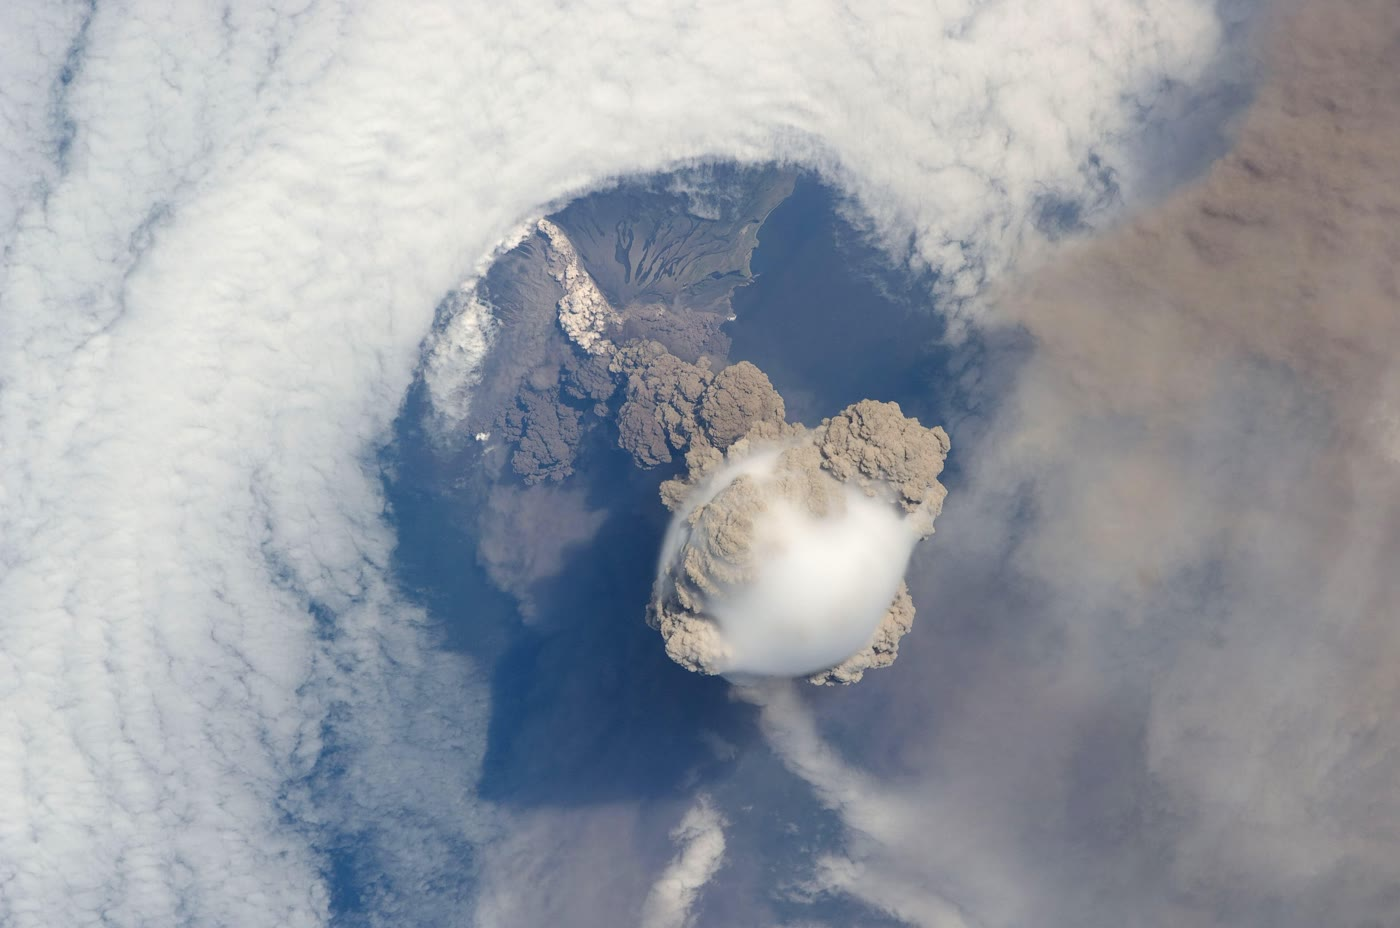
\includegraphics[width=0.66\linewidth]{images/book3/b1-sarychev-iss.jpg}
\par\smallskip{\small सारिचेव शिखर, मातुआ द्वीप पर कुरील चाप का एक ज्वालामुखी, 12 जून 2009 को विस्फोट के आरंभिक चरण में, अंतर्राष्ट्रीय अंतरिक्ष स्टेशन से बादलों के एक छेद से देखा गया। शिखर से भूरी राख, संभवतः एक पाइरोक्लास्टिक प्रवाह, नीचे आती है, और उठते स्तंभ पर एक चिकनी बादल-टोपी, एक पिलियस, बैठी है; विस्फोट की राख \qty{2400}{km} से अधिक दूर पाई गई। फ़ोटो: NASA, सार्वजनिक क्षेत्र (Wikimedia Commons)।}
\label{fig:b1:active-margins:sarychev}
\end{omfigure}
% ledger: nasa:sarychev, commons:sarychev

आर्क के नीचे की \omterm{def:b1:layered-earth:layers}{भूपर्पटी} छोटा होने और ऊपर से जोड़े गए मैग्मा दोनों से मोटी है; आंडीज़ जैसे महाद्वीपों पर बने चापों के नीचे वह पृथ्वी की सबसे मोटी भूपर्पटियों में से है।

कुछ चापों के पीछे ऊपरी प्लेट खींची जाती है। डैन कैरिग ने 1971 में पश्चिमी प्रशांत की इन सीमांत द्रोणियों को प्लेट विवर्तनिकी के भीतर समझाया: जब स्लैब तीखा धँसता है और पीछे लौटता है, तो खाई और चाप धँसती प्लेट की ओर खिसकते हैं, और उनके पीछे की प्लेट तब तक खिंचती है जब तक वह टूट न जाए, कभी दूसरी ओर एक विलुप्त अवशेष चाप छोड़ते हुए। ऊपर प्रयुक्त प्लेट प्रतिरूप में, बैक-आर्क प्रसार लगभग \qty{32}{mm.yr^{-1}} पर मारियाना ट्रफ़ में \ang{18}\,N के निकट चलता है, और टोंगा के पीछे लाउ द्रोणी के उत्तर में \qty{110}{mm.yr^{-1}} से अधिक पर। जहाँ स्लैब उथला है, इसके विपरीत, वह ऊपरी प्लेट को खींचता है, जिसकी \omterm{def:b1:layered-earth:layers}{भूपर्पटी} चाप के पीछे छोटी और मोटी होती है, जैसे आंडीज़ के पीछे।
% ledger: karig:marginal-basins, data:pb2002 (ridge_budget.py: Mariana 32.4, Lau 117.5 mm/yr)

\begin{inthefield}[सुनामी चेतावनी]
एक सुनामी चेतावनी केंद्र के पास मिनट होते हैं। 2011 में उत्तर-पूर्वी जापान के तट के लिए पहली चेतावनी भूकंप के लगभग तीन मिनट बाद आई, छोटी-अवधि की भूकंपीय तरंगों पर आधारित परिमाण से; परिमाण 8 या उससे अधिक के भूकंपों के लिए ऐसा परिमाण कम आँका जाता है, और सुनामी की ऊँचाई भी कम आँकी गई। आघूर्ण परिमाण, जो संतृप्त नहीं होता, लगभग पंद्रह मिनट में आया: जापान के चौड़े-बैंड भूकंपमापी अपनी सीमा से परे धकेले गए थे। 2013 से, जब इतने बड़े भूकंप का आकार अनिश्चित हो, पहली चेतावनी वहाँ संभव सबसे बड़ा भूकंप मानती है और सुनामी को संख्या के बजाय शब्दों में वर्णित करती है, जैसे ``विशाल'', और पूर्वानुमान समुद्र के अपने तट-दूर मापों पर आधारित होते हैं: उपग्रह से स्थित बॉय और समुद्र-तल के दबाव-गेज, जो लहर को तट तक पहुँचने से पहले देखते हैं।
% ledger: jma:warning

\smallskip
\begin{center}
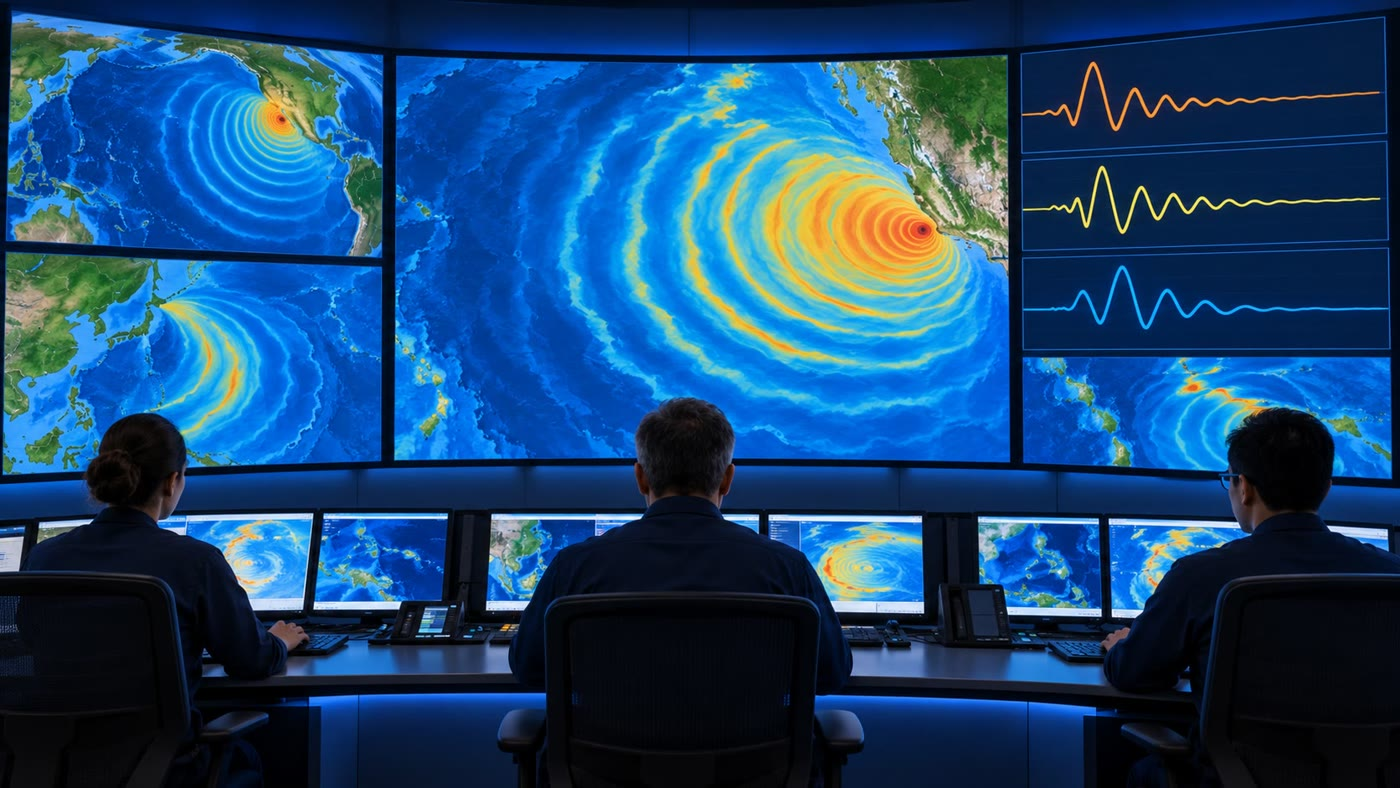
\includegraphics[width=0.7\linewidth]{images/book3/ai/b1-tsunami-centre.jpg}

{\scriptsize सुनामी चेतावनी केंद्र में ड्यूटी अधिकारी, परिकलित तरंग-मोर्चों और समुद्र-स्तर के रिकॉर्डों के पर्दों के सामने (AI से बनाया गया चित्र)।}
\end{center}
\end{inthefield}

\section{अभ्यास}

\begin{exercise}[$\star$]\label{exo:b1:active-margins:1}
एक खाई उसके चारों ओर के समुद्र-तल से \qty{3}{km} नीचे है। (क) यदि वह प्रतिपूरित नहीं होती, तो \qty{1000}{kg.m^{-3}} घनत्व के समुद्री पानी से बदले गए, \qty{2700}{kg.m^{-3}} घनत्व के अनुपस्थित चट्टान, वहाँ गुरुत्व को कितना कम करते? बूगेर पट्टी का प्रयोग कीजिए, $G = \qty{6.674e-11}{m^3.kg^{-1}.s^{-2}}$ के साथ। (ख) कुरील खाई पर प्रेक्षित विसंगति, लगभग \qty{-260}{\milli\gal}, से तुलना कीजिए, जहाँ खाई अपने चारों ओर के तल से \qty{3.5}{km} नीचे है: उस गहराई के लिए परिकलन दोहराइए। (ग) दसियों किलोमीटर चौड़ी खाई में पानी स्लैब सूत्र से कम क्यों देता है, और कमी का शेष भाग कहाँ होना चाहिए?
\end{exercise}

\begin{exercise}[$\star$]\label{exo:b1:active-margins:2}
पैसिफ़िक प्लेट कुरील खाई में \qty{82}{mm.yr^{-1}} पर प्रवेश करती है। (क) 10 मिलियन वर्षों में कितनी प्लेट नीचे जाती है? (ख) यदि स्लैब \ang{45} \omterm{def:b1:geological-maps:attitude}{नति} वाले एक सीधे पथ के अनुदिश धँसे, तो उसका अग्रणी किनारा तब कितना गहरा होगा? (ग) \qty{600}{km} तक पहुँचने में कितना समय लगता है?
\end{exercise}

\begin{exercise}[$\star$]\label{exo:b1:active-margins:3}
सीधा स्लैब जहाँ \qty{110}{km} गहरा है, वहाँ के ऊपर ज्वालामुखी खड़े हैं। \ang{30}, \ang{45} और \ang{60} \omterm{def:b1:geological-maps:attitude}{नति} वाले स्लैब के लिए \omterm{def:b1:active-margins:volcanic-arc}{चाप–खाई अंतराल} परिकलित कीजिए। कौन-सा चाप अपनी खाई से सबसे दूर है?
\end{exercise}

\begin{exercise}[$\star$]\label{exo:b1:active-margins:4}
अध्याय के अंकीय प्लेट प्रतिरूप में, हर वर्ष लगभग \qty{2.7}{km^2} महासागर-तल \qty{51000}{km} के साथ निमज्जन-सीमाओं से नीचे जाता है, और लगभग \qty{3.0}{km^2} लगभग \qty{67000}{km} प्रसारी कटकों पर बनता है। (क) माध्य अभिसरण-दर और माध्य \omterm{def:b1:plate-kinematics:spreading-rate}{पूर्ण प्रसार-दर}, \unit{mm.yr^{-1}} में परिकलित कीजिए। (ख) अपनी सभी सीमाओं पर प्रतिरूप उतना ही क्षेत्र नष्ट करता है जितना बनाता है। नए तल का बाकी भाग कहाँ जाता है?
% ledger: data:pb2002 (ridge_budget.py: 2.739 km2 over 51471 km; 3.009 km2 over 67340 km; all 3.511 vs 3.519)
\end{exercise}

\begin{exercise}[$\star\star$]\label{exo:b1:active-margins:5}
एक खंड के चार भूकंप $(x, z) = (200, 150)$, $(300, 250)$, $(400, 330)$ और $(500, 430)$ पर हैं, किलोमीटर में। (क) न्यूनतम वर्गों से स्लैब की रेखा फ़िट कीजिए और उसकी \omterm{def:b1:geological-maps:attitude}{नति} दीजिए। (ख) रेखा सतह तक कहाँ पहुँचती है? (ग) केवल पहले और अंतिम भूकंपों से होकर जाने वाली रेखा की \omterm{def:b1:geological-maps:attitude}{नति} से तुलना कीजिए।
\end{exercise}

\begin{exercise}[$\star\star$]\label{exo:b1:active-margins:6}
एक प्रतिरूप स्लैब खाई से \qty{50}{km} तक \ang{25} \omterm{def:b1:geological-maps:attitude}{नति} पर झुकता है, फिर \ang{45}। ज्वालामुखी अग्र वहाँ है जहाँ स्लैब \qty{110}{km} गहरा है। (क) \omterm{def:b1:active-margins:volcanic-arc}{चाप–खाई अंतराल} परिकलित कीजिए। (ख) पूरे रास्ते \ang{45} \omterm{def:b1:geological-maps:attitude}{नति} वाले स्लैब से तुलना कीजिए। (ग) गहरा खंड, ऊपर की ओर बढ़ाया गया, सतह तक पहुँचता है: कहाँ? कुरील रेखा से तुलना कीजिए, जो उस तक खाई से \qty{53}{km} भू-ओर पहुँचती है। (घ) \ang{60} के गहरे खंड से कौन-सा अंतराल मिलेगा?
\end{exercise}

\begin{exercise}[$\star\star$]\label{exo:b1:active-margins:7}
(क) मुड़े-कवच प्रस्ताव के द्वारा, \ang{45} \omterm{def:b1:geological-maps:attitude}{नति} वाले स्लैब के ऊपर एक चाप की कौन-सी कोणीय त्रिज्या, और किलोमीटर में कौन-सी त्रिज्या ($R = \qty{6371}{km}$), होनी चाहिए? \ang{30}? \ang{70}? (ख) कौन-से चाप सबसे कसकर मुड़े हैं? (ग) कुरील स्लैब \ang{44.9} \omterm{def:b1:geological-maps:attitude}{नति} पर झुकता है और कुरील खाई \ang{21.9} के एक वृत्त से फ़िट होती है: पूर्वानुमान से सापेक्ष अंतर परिकलित कीजिए।
\end{exercise}

\begin{exercise}[$\star\star$]\label{exo:b1:active-margins:8}
चालकता \qty{2.5}{W.m^{-1}.K^{-1}} और सतह-तापमान \qty{10}{\celsius} लीजिए। (क) \qty{35}{mW.m^{-2}} खोते \omterm{def:b1:active-margins:active-margin}{फ़ोरआर्क} के नीचे और \qty{80}{mW.m^{-2}} खोते बैक-आर्क के नीचे सतह तापमान प्रवणता परिकलित कीजिए। (ख) इन प्रवणताओं को रैखिक रूप से बढ़ाकर, हर एक में \qty{30}{km} पर तापमान का अनुमान लगाइए। (ग) बैक-आर्क \omterm{def:b1:layered-earth:discontinuity}{मोहो} 800 से \qty{900}{\celsius} पर मापे गए हैं। रैखिक अनुमान बहुत अधिक क्यों है?
% ledger: hyndman:backarc (back-arc 70-85, Moho 800-900); the forearc value is an exercise value
\end{exercise}

\begin{exercise}[$\star\star$]\label{exo:b1:active-margins:9}
अध्याय के प्लेट प्रतिरूप में, मारियाना ट्रफ़ \ang{18}\,N के निकट लगभग \qty{32}{mm.yr^{-1}} की पूर्ण दर पर खुलता है। (क) इस दर को \unit{km.Myr^{-1}} में व्यक्त कीजिए, और यदि प्रसार सममित हो तो अर्ध दर दीजिए। (ख) इस दर पर ट्रफ़ को \qty{100}{km} खुलने में कितना समय लगेगा? (ग) दो कारण दीजिए कि किसी \omterm{def:b1:active-margins:active-margin}{बैक-आर्क द्रोणी} की आयु उसकी चौड़ाई और उसकी वर्तमान दर से सरलता से क्यों नहीं पढ़ी जा सकती।
% ledger: data:pb2002 (ridge_budget.py: mariana_18n_mm_yr 32.4)
\end{exercise}

\begin{exercise}[$\star\star\star$]\label{exo:b1:active-margins:10}
\qty{100}{km} मोटा एक स्लैब \ang{45} \omterm{def:b1:geological-maps:attitude}{नति} वाले पथ के अनुदिश \qty{82}{mm.yr^{-1}} पर धँसता है। $\kappa = \qty{e-6}{m^2.s^{-1}}$ लीजिए। (क) \qty{600}{km} तक पहुँचने में कितना समय लगता है? (ख) उस समय में ऊष्मा $\sqrt{\kappa t}$ से उसमें कितनी दूर विसरित होती है? (ग) ऊष्मा को उसके मध्य तक पहुँचने में कितना समय लगेगा? (घ) \qty{600}{km} पर स्लैब के तापमान और उसके भूकंपों के बारे में निष्कर्ष निकालिए।
\end{exercise}

\begin{exercise}[$\star\star\star$]\label{exo:b1:active-margins:11}
एक मॉडल \omterm{def:b1:active-margins:accretionary}{संचयी प्रिज़्म} का त्रिकोणीय काट है: उसकी सतह खाई की ओर $\alpha = \ang{4}$ पर ढलती है और उसका आधार उसके नीचे $\beta = \ang{6}$ पर झुकता है, दोनों उसके पैर पर मिलते हुए; वह बढ़ते हुए ये कोण बनाए रखता है। (क) दिखाइए कि उसका क्षेत्रफल $A = \frac12 L^2(\tan\alpha + \tan\beta)$ है, चौड़ाई $L$ के लिए, जब कोण इतने छोटे हों कि पिछली ओर की ऊँचाई $L(\tan\alpha + \tan\beta)$ हो। (ख) \qty{1}{km} मोटा अवसाद \qty{40}{mm.yr^{-1}} पर अभिसरित होती प्लेट पर पहुँचता है, और उसका सब कुछ संचित होता है: 1, 4 और 10 मिलियन वर्ष बाद चौड़ाई परिकलित कीजिए। $L$ समय के साथ कैसे बढ़ता है? (ग) यदि आधा अवसाद स्लैब के साथ नीचे चला जाए तो क्या होगा?
\end{exercise}

\begin{exercise}[$\star\star\star$]\label{exo:b1:active-margins:12}
(क) दिखाइए कि न्यूनतम-वर्ग रेखा माध्य बिंदु $(\bar x, \bar z)$ से होकर जाती है। (ख) एक सूची हर गहराई को \qty{10}{km} बहुत गहरा सूचीबद्ध करती है। फ़िट रेखा की ढलान और अंतःखंड कैसे बदलते हैं? (ग) दूरियाँ $x$ सभी एक खाई-बिंदु से मापी गई हैं जो \qty{20}{km} बहुत भू-ओर रखा गया है, अतः हर $x$ \qty{20}{km} बहुत छोटा है। ढलान और अंतःखंड कैसे बदलते हैं? (घ) क्या कोई त्रुटि \omterm{def:b1:geological-maps:attitude}{नति} बदलती है?
\end{exercise}

\section{समस्या: एक निमज्जन-क्षेत्र को उसके भूकंपों से पढ़ना}

\begin{problem}[{सप्ताहांत समस्या --- आठ भूकंपों से कुरील स्लैब, वह कितनी तेज़ी से नीचे जाता है, उसका गुरुत्व और ऊष्मा-प्रवाह क्या कहते हैं, और उसके ज्वालामुखी कहाँ खड़े होने चाहिए}]
\label{pb:b1:active-margins:1}
% values: calc/ch14.py; the eight events are real (USGS catalogue, rounded to the km)
% from figdata/out/bachelor-1-slab_seismicity-section.dat
% ledger: data:b3-usgs-kuril, data:pb2002, data:b2-seafloor-age, syracuse:arc-depth, frank:arcs,
% data:b3-grav-kuril, parsons:plate-model, hyndman:backarc; the forearc heat flow is an exercise value
कुरील स्लैब के आठ भूकंप, सभी \qty{70}{km} से गहरे, परिच्छेद रेखा के साथ खाई से उनकी दूरी $x$, ओखोत्स्क सागर की ओर, और उनकी गहराई $z$ से सूचीबद्ध हैं, दोनों किलोमीटर तक पूर्णांकित।

\begin{center}
\small
\begin{tabular}{lcccccccc}
\hline
घटना & 1 & 2 & 3 & 4 & 5 & 6 & 7 & 8\\
$x$ (\unit{km}) & 155 & 222 & 305 & 319 & 431 & 533 & 578 & 609\\
$z$ (\unit{km}) & 96 & 169 & 245 & 272 & 389 & 489 & 518 & 573\\
परिमाण & 5.5 & 5.1 & 5.0 & 5.4 & 5.3 & 5.3 & 5.2 & 6.4\\
\hline
\end{tabular}
\end{center}

\medskip
\noindent\textbf{भाग I --- स्लैब की रेखा।}
\begin{enumerate}
  \item सभी आठ भूकंपों को दोनों अक्षों पर एक ही पैमाने पर, गहराई नीचे की ओर, अंकित कीजिए।
  \item $\sum x_i$, $\sum z_i$, $\sum x_i^2$, $\sum x_i z_i$ और माध्य $\bar x$ और $\bar z$ परिकलित कीजिए।
  \item $S_{xx}$ और $S_{xz}$ परिकलित कीजिए, फिर न्यूनतम-वर्ग रेखा की ढलान तीन दशमलव तक और उसका अंतःखंड एक दशमलव तक।
  \item स्लैब की \omterm{def:b1:geological-maps:attitude}{नति} क्या है?
  \item रेखा सतह तक कहाँ पहुँचती है? खाई के निकट स्लैब के आकार के बारे में यह क्या कहता है?
  \item हर भूकंप का विचलन $z_i - (a + s x_i)$ परिकलित कीजिए। कौन-से रेखा से सबसे दूर हैं, और कितना दूर?
\end{enumerate}

\medskip
\noindent\textbf{भाग II --- स्लैब कितनी तेज़ी से नीचे जाता है।} परिच्छेद के आरंभ पर PB2002 प्रतिरूप \qty{87.4}{mm.yr^{-1}} का अभिसरण देता है: ओखोत्स्क प्लेट के सापेक्ष, पैसिफ़िक प्लेट दिगंश \ang{300} की ओर चलती है। परिच्छेद रेखा, खाई के लंबवत, दिगंश \ang{320.9} की ओर चलती है।
\begin{enumerate}[resume]
  \item अभिसरण और परिच्छेद रेखा के बीच का कोण परिकलित कीजिए, फिर खाई के लंबवत और समांतर अभिसरण के घटक।
  \item 10 मिलियन वर्षों में खाई से कितनी लंबाई की प्लेट नीचे जाती है?
  \item प्रश्न 4 की \omterm{def:b1:geological-maps:attitude}{नति} का प्रयोग करते हुए (\ang{45} तक पूर्णांकित), स्लैब के शीर्ष के एक बिंदु को खाई से पट्टी के सबसे गहरे भूकंप, \qty{632}{km}, तक ले जाने में कितना समय लगता है? खाई के निकट की मंद \omterm{def:b1:geological-maps:attitude}{नति} की उपेक्षा कीजिए।
  \item खाई पर प्लेट लगभग \qty{122}{Myr} पुरानी है। अब \qty{632}{km} गहरा समुद्र-तल कितना पुराना है?
  \item $\sqrt{\kappa t}$ से, $\kappa = \qty{e-6}{m^2.s^{-1}}$ के साथ, उस अवतरण के दौरान ऊष्मा स्लैब में कितनी दूर विसरित हुई है? उसकी मोटाई, लगभग \qty{100}{km}, से तुलना कीजिए।
\end{enumerate}

\medskip
\noindent\textbf{भाग III --- गुरुत्व और ऊष्मा-प्रवाह।} चालकता \qty{2.5}{W.m^{-1}.K^{-1}} लीजिए।
\begin{enumerate}[resume]
  \item खाई के सामने का पुराना महासागर-तल लगभग \qty{43}{mW.m^{-2}} खोता है, बैक-आर्क लगभग \qty{80}{mW.m^{-2}}; \omterm{def:b1:active-margins:active-margin}{फ़ोरआर्क} के लिए \qty{35}{mW.m^{-2}} लीजिए। हर एक के सतह के निकट तापमान प्रवणता परिकलित कीजिए।
  \item समझाइए कि \omterm{def:b1:active-margins:active-margin}{फ़ोरआर्क} सामने के पुराने महासागर-तल से कम ऊष्मा क्यों खोता है।
  \item कुरील खाई पर \omterm{def:b1:isostasy-gravity:anomalies}{मुक्त-वायु विसंगति} लगभग \qty{-260}{\milli\gal} है। कितनी चट्टान की मोटाई, जो पानी से \qty{1700}{kg.m^{-3}} सघन है, एक बूगेर पट्टी को यह कमी देने के लिए चाहिए? उसकी तुलना उसके चारों ओर के तल से खाई की गहराई, लगभग \qty{3.5}{km}, से कीजिए।
  \item अब मान लीजिए पूरी प्लेट \qty{3.5}{km} नीचे धकेली गई है: पानी उसके शीर्ष पर चट्टान का स्थान लेता है, और उसकी \omterm{def:b1:layered-earth:layers}{भूपर्पटी} उसके आधार पर \omterm{def:b1:layered-earth:layers}{प्रावार} का स्थान लेती है, अतः, कुल मिलाकर, \qty{3300}{kg.m^{-3}} घनत्व का \omterm{def:b1:layered-earth:layers}{प्रावार} पानी से बदल दिया जाता है। बूगेर स्लैब विसंगति परिकलित कीजिए। वास्तविक खाई, जो केवल दसियों किलोमीटर चौड़ी है, कम क्यों देती है?
  \item खाई और बाहरी उभार समस्थैतिक साम्य में नहीं हैं। उन्हें उससे बाहर क्या रखता है?
\end{enumerate}

\medskip
\noindent\textbf{भाग IV --- ज्वालामुखी कहाँ खड़े होने चाहिए।} प्रश्न 3 की रेखा का प्रयोग कीजिए, उसकी पूर्णांकित ढलान और अंतःखंड के साथ।
\begin{enumerate}[resume]
  \item पट्टी का पहला ज्वालामुखी खाई से \qty{164}{km} पर है। उसके नीचे स्लैब कितना गहरा है?
  \item क्या यह गहराई चापों के नीचे पाई गई सीमा, \qty{72} से \qty{173}{km}, के भीतर है? औसत, \qty{105}{km}, से यह कितनी दूर है?
  \item खाई से किस दूरी पर स्लैब \qty{100}{km} गहरा है?
  \item मुड़े-कवच प्रस्ताव के द्वारा, कुरील चाप की कौन-सी कोणीय त्रिज्या, और किलोमीटर में कौन-सी त्रिज्या, होनी चाहिए?
  \item कुरील खाई \ang{21.9} के एक लघुवृत्त से फ़िट होती है। तुलना कीजिए।
  \item चाप के ज्वालामुखी औसतन वहाँ खड़े होते हैं जहाँ स्लैब लगभग \qty{105}{km} गहरा है। खाई से किस दूरी पर स्लैब रेखा वह गहराई पहुँचती है?
  \item इस दूरी की प्रेक्षित \qty{164}{km} से तुलना कीजिए: कितने किलोमीटर और किस अंश से वह भिन्न है?
  \item किलोमीटर के निकटतम, कुरील स्लैब रेखा किस \omterm{def:b1:active-margins:volcanic-arc}{चाप–खाई अंतराल} का अनुमान लगाती है, \qty{105}{km} पर स्लैब के ऊपर खड़े ज्वालामुखियों के लिए?
\end{enumerate}
\end{problem}
